The simulation consists of two parts:
\vspace{-5pt}
\begin{itemize}
	\item[(1)] \textbf{Generate theoretical curve \hfill \\}
	Generate the theoretical curve under different $L$ and SNR by
	\begin{equation*}
		C_{\epsilon, \text{theoretical}} = \log\left(1 + F^{-1}(1-\epsilon) \, \text{SNR}\right)
	\end{equation*}
	where $F(x) = P\left(\|h\|^{2} > x\right)$ and $\|h\|^{2}$ is chi-square distribution with $2L$ degrees of freedom.
	\item[(2)] \textbf{Generate Simulated curve \hfill \\}
	To generate the simulated curve, recall the definition of $\epsilon$-outage probability:
	\begin{equation*}
		\epsilon\left(C\right) = P\left(\log(1 + \|h\|^{2} \, \text{SNR}) < C\right)
	\end{equation*} 
	Given $\epsilon$, $L$, and SNR, we first generate a large number ($N = 10^6$) of channel 
	realizations from a chi-square distribution with $2L$ degrees of freedom. Calculate 
	$\log(1 + \|h\|^{2} \, \text{SNR})$ for each realization and sort them into nondecreasing 
	order. Let $k = N\epsilon$, and pick the $k$th smallest value from the sorted data, which
	 is then the simulated result.

\end{itemize}

The comparison between theoretical computation and simulation is shown below. Solid lines 
represent the theoretical result and marked points show the simulated result. 
\begin{figure}[H]
	\centering
	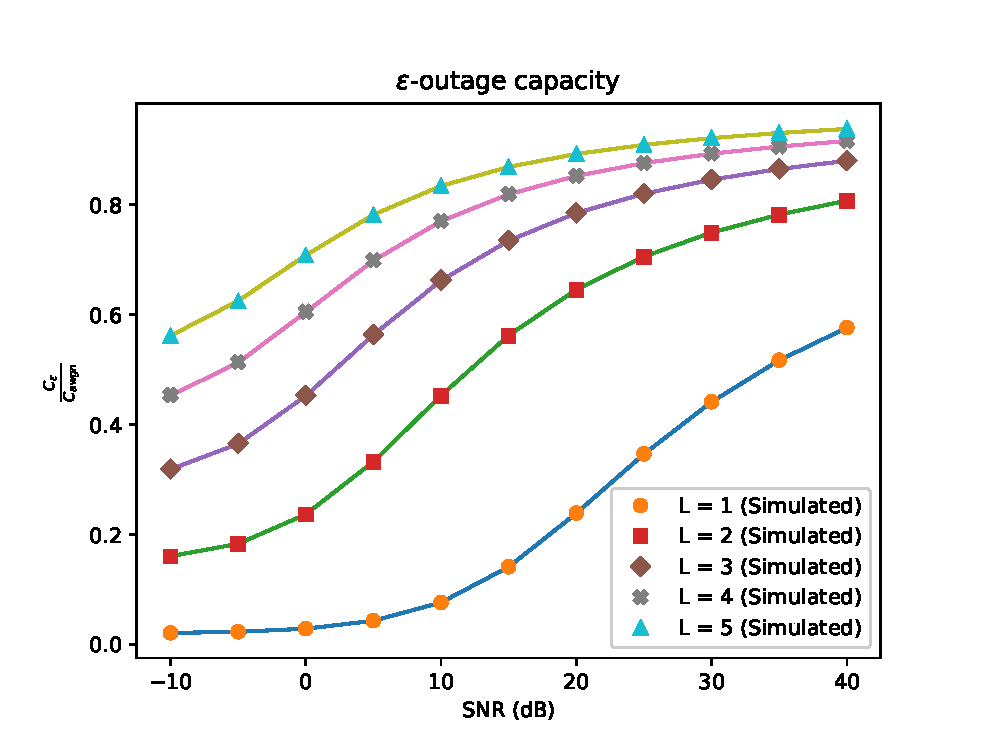
\includegraphics[scale = 0.85]{epsilon_outage.eps}
\end{figure}